% Options for packages loaded elsewhere
\PassOptionsToPackage{unicode}{hyperref}
\PassOptionsToPackage{hyphens}{url}
%
\documentclass[
  11pt,
]{article}
\usepackage{amsmath,amssymb}
\usepackage{lmodern}
\usepackage{iftex}
\ifPDFTeX
  \usepackage[T1]{fontenc}
  \usepackage[utf8]{inputenc}
  \usepackage{textcomp} % provide euro and other symbols
\else % if luatex or xetex
  \usepackage{unicode-math}
  \defaultfontfeatures{Scale=MatchLowercase}
  \defaultfontfeatures[\rmfamily]{Ligatures=TeX,Scale=1}
  \setmainfont[Scale=MatchLowercase]{SF Pro Text Light}
\fi
% Use upquote if available, for straight quotes in verbatim environments
\IfFileExists{upquote.sty}{\usepackage{upquote}}{}
\IfFileExists{microtype.sty}{% use microtype if available
  \usepackage[]{microtype}
  \UseMicrotypeSet[protrusion]{basicmath} % disable protrusion for tt fonts
}{}
\makeatletter
\@ifundefined{KOMAClassName}{% if non-KOMA class
  \IfFileExists{parskip.sty}{%
    \usepackage{parskip}
  }{% else
    \setlength{\parindent}{0pt}
    \setlength{\parskip}{6pt plus 2pt minus 1pt}}
}{% if KOMA class
  \KOMAoptions{parskip=half}}
\makeatother
\usepackage{xcolor}
\usepackage[margin=1in]{geometry}
\usepackage{graphicx}
\makeatletter
\def\maxwidth{\ifdim\Gin@nat@width>\linewidth\linewidth\else\Gin@nat@width\fi}
\def\maxheight{\ifdim\Gin@nat@height>\textheight\textheight\else\Gin@nat@height\fi}
\makeatother
% Scale images if necessary, so that they will not overflow the page
% margins by default, and it is still possible to overwrite the defaults
% using explicit options in \includegraphics[width, height, ...]{}
\setkeys{Gin}{width=\maxwidth,height=\maxheight,keepaspectratio}
% Set default figure placement to htbp
\makeatletter
\def\fps@figure{htbp}
\makeatother
\setlength{\emergencystretch}{3em} % prevent overfull lines
\providecommand{\tightlist}{%
  \setlength{\itemsep}{0pt}\setlength{\parskip}{0pt}}
\setcounter{secnumdepth}{-\maxdimen} % remove section numbering
% https://github.com/rstudio/rmarkdown/issues/337
\let\rmarkdownfootnote\footnote%
\def\footnote{\protect\rmarkdownfootnote}

% https://github.com/rstudio/rmarkdown/pull/252
\usepackage{titling}
\setlength{\droptitle}{-2em}

\pretitle{\vspace{\droptitle}\centering\huge}
\posttitle{\par}

\preauthor{\centering\large\emph}
\postauthor{\par}

\predate{\centering\large\emph}
\postdate{\par}

\usepackage[normalem]{ulem}
\usepackage{nicefrac}
\usepackage{caption}
\usepackage{multicol}
\ifLuaTeX
  \usepackage{selnolig}  % disable illegal ligatures
\fi
\IfFileExists{bookmark.sty}{\usepackage{bookmark}}{\usepackage{hyperref}}
\IfFileExists{xurl.sty}{\usepackage{xurl}}{} % add URL line breaks if available
\urlstyle{same} % disable monospaced font for URLs
\hypersetup{
  pdftitle={Assignment Week 7},
  pdfauthor={Philosophy 444},
  hidelinks,
  pdfcreator={LaTeX via pandoc}}

\title{Assignment Week 7}
\author{Philosophy 444}
\date{Due 17 February, 2023}

\begin{document}
\maketitle

\pagenumbering{gobble}

You have a choice of assignments this week. You can either answer some
numerical questions from chapter 7 of Bonanno, or do a (very) short
essay. \textbf{Do not do both!}. You \textbf{either} do the 12 questions
from the numerical track, \textbf{or} the essay question.

\hypertarget{numerical-track}{%
\section{Numerical Track}\label{numerical-track}}

These questions all concern variants of the game tree on page 246 of
Bonanno. It's the game tree for question 7.7, and the basic case is
repeated here. (Looking over the answers to question 7.7 may be very
helpful in working out these problems.)

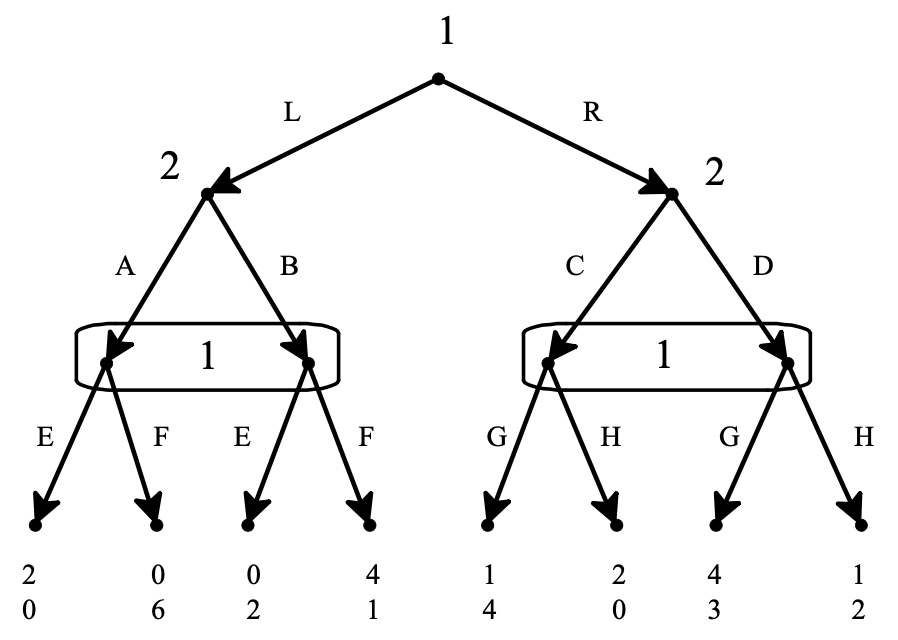
\includegraphics[width=0.75\textwidth,height=\textheight]{bonanno-tree.png}

\hypertarget{questions-1-4}{%
\subsection{Questions 1-4}\label{questions-1-4}}

Change the payoffs of the game to replace every value of 4 with -4. So
if player 1 plays L, then player 2 plays B, then player 1 plays F, the
outcome is no longer 4, 1; it's -4, 1.

\begin{enumerate}
\def\labelenumi{\arabic{enumi}.}
\tightlist
\item
  How many pure-strategy Nash equilibria are there in this variant of
  the game?
\item
  In the (possibly mixed) subgame-perfect equilibrium of this variant of
  the game, does 1 play L or R?
\item
  In the (possibly mixed) subgame-perfect equilibrium of this variant of
  the game, what is player 1's expected return?
\item
  In the (possibly mixed) subgame-perfect equilibrium of this variant of
  the game, what is player 2's expected return?
\end{enumerate}

\hypertarget{questions-5-8}{%
\subsection{Questions 5-8}\label{questions-5-8}}

Change the payoffs of the game to replace every value of 4 with 3. So if
player 1 plays L, then player 2 plays B, then player 1 plays F, the
outcome is no longer 4, 1; it's 3, 1.

\begin{enumerate}
\def\labelenumi{\arabic{enumi}.}
\setcounter{enumi}{4}
\tightlist
\item
  How many pure-strategy Nash equilibria are there in this variant of
  the game?
\item
  In the (possibly mixed) subgame-perfect equilibrium of this variant of
  the game, does 1 play L or R?
\item
  In the (possibly mixed) subgame-perfect equilibrium of this variant of
  the game, what is player 1's expected return?
\item
  In the (possibly mixed) subgame-perfect equilibrium of this variant of
  the game, what is player 2's expected return?
\end{enumerate}

\hypertarget{questions-9-12}{%
\subsection{Questions 9-12}\label{questions-9-12}}

Change the payoffs of the game by switching what player 1 and player 2
get in each outcome. So if player 1 plays L, then player 2 plays B, then
player 1 plays F, the outcome is no longer 4, 1; it's 1, 4.

\begin{enumerate}
\def\labelenumi{\arabic{enumi}.}
\setcounter{enumi}{8}
\tightlist
\item
  How many pure-strategy Nash equilibria are there in this variant of
  the game.
\item
  In the (possibly mixed) subgame-perfect equilibrium of this variant of
  the game, does 1 play L or R?
\item
  In the (possibly mixed) subgame-perfect equilibrium of this variant of
  the game, what is player 1's expected return?
\item
  In the (possibly mixed) subgame-perfect equilibrium of this variant of
  the game, what is player 2's expected return?
\end{enumerate}

\hypertarget{essay-track}{%
\section{Essay Track}\label{essay-track}}

Write 600-800 words (no more), on the following questions.

Very briefly describe the Spence signalling model of why people go into
higher education, and why employers pay a premium for college graduates.
As an explanation of the wage premium that college graduates receive,
what about it is most plausible? And what about it is least plausible?
(In the space you've got, you won't really be able to \emph{defend}
these claims about plausibility - I just want you to identify a strength
and a weakness of the model.)

\end{document}
